\documentclass{article}
\usepackage[T1]{fontenc}
\usepackage{lmodern}
\usepackage{graphicx}
\usepackage{amsmath,amssymb}
\usepackage[a4paper,margin=2cm]{geometry}
\usepackage[absolute,overlay]{textpos}
\setlength{\TPHorizModule}{1mm}
\setlength{\TPVertModule}{1mm}
\usepackage[indonesian]{babel}
\usepackage{hyperref}
\setlength{\emergencystretch}{2em}
% unit: Halaman 41

\begin{document}

% === Halaman 41 (python/native) ===

Citra Digital

• Citra terdiri dari sejumlah pixel. Citra 1200 x 1500 berarti memiliki 1200 x 1500 pixel = 

1.800.000 pixel

• Setiap pixel panjangnya n-bit. 

 Citra biner → 1 bit/pixel

 Citra grayscale → 8 bit/pixel

 Citra true color → 24 bit/pixel

41

pixel

% deskripsi: gambar native xref 201
\noindent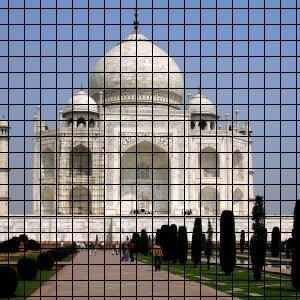
\includegraphics[width=0.85\textwidth]{../../images/python/page_041_img_01.jpeg}

% deskripsi: gambar native xref 202
\noindent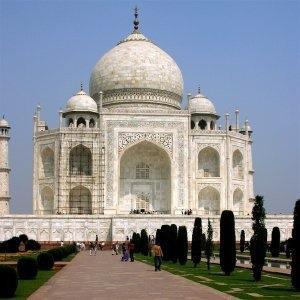
\includegraphics[width=0.85\textwidth]{../../images/python/page_041_img_02.jpeg}

\end{document}
